%!TEX root = ../main.tex

\subsection{Tau}
360 is nice enough number.  It divides evenly by 2, 3, 4, 5, 6, 8, 9, 10, 12, 15, 18, 20, 24, 30,
36, 40, 45, 60, 72, 90, and 180.  No other number under 1000 even comes close.  But it
is still arbitrary.  Why are there 60 seconds in a minute, 60 minutes in an hour, 360 degrees
in a full rotation?  Because Babylonian mathematicians wanted numbers that were easier
division!

A far more natural system exists and is indeed the only one used in calculus and higher
mathematics today.  Rather than assigning an arbitrary number to the complete
circle, we ask instead, what fraction of a full rotation have you turned?  One full rotation
will correspond with the entire circumference of the circle.  And again, this will be
done on the Unit Circle, so that an angle's measure is defined as the arc length
divided by the radius.  Because this is length divided by length, angles in this system
(called radians) have no units.  Turning all the way around one time is the same as
laying the radius of any circle out in a curved piece $6.28\dots$ times.  Rather than
write this irrational number to some arbitrary number of decimals, we use the symbol
$\tau$, called TAU.

There are no calculators with the number $\tau$ on them (yet), so we must use 
the fact that $\tau=2\pi$.

\subsection{Unit Circle}
This all culminates in the single figure that most embodies trigonometry: the completed
Unit Circle.  Because your education up to this point has utilized degrees, they are included
but you should concentrate on using radians, as they will be the main system used
from now on.  

\begin{figure}
\begin{center}
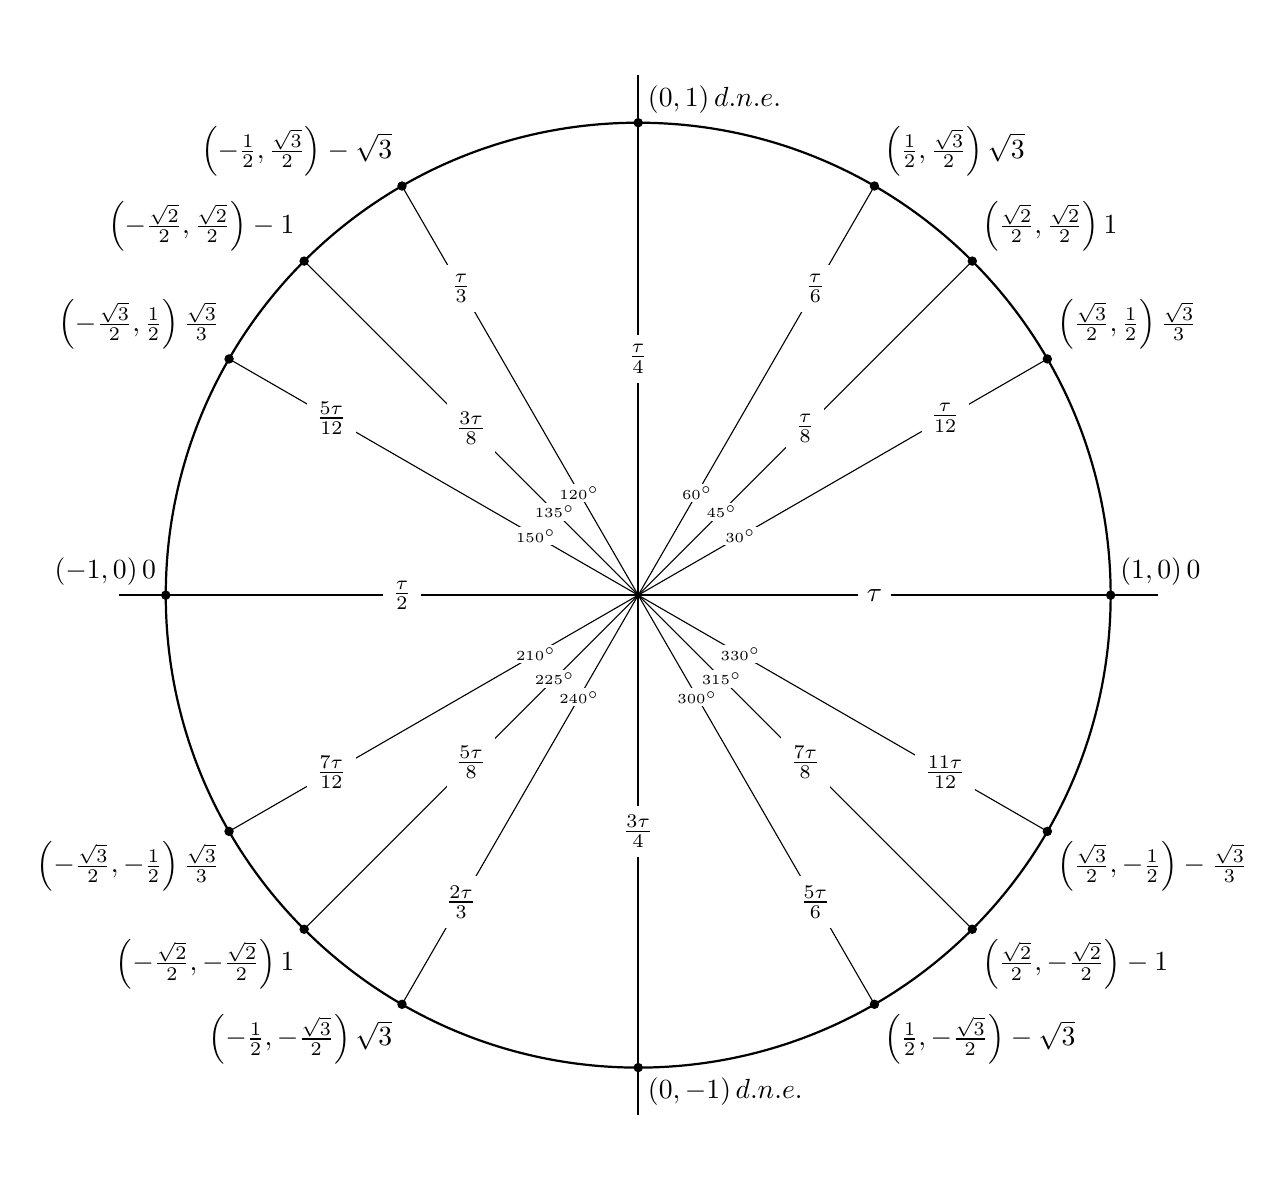
\begin{tikzpicture} [scale=2,
% Toggle commenting on the next four lines for the completed unit circle:
angle/.style={draw,text=white,fill=white,minimum height=1cm, minimum width=1cm},
point/.style={white},
angle/.style={fill=white},
point/.style={},
]
    \draw [white] (-3.6,-3.6) rectangle (3.6,3.6);
    \draw [thick,fill=white] (0,0) circle (3cm);
    \draw [thick, ] (-3.3,0) -- (3.3,0);
    \draw [thick, ] (0,-3.3) -- (0,3.3);
    \draw (0,0) --  node [angle] {$\frac{\tau}{4}$} (90:3)
                node[point, above right] {$ \left(0,1\right)  d.n.e.$};
    \draw (0,0) --  node [angle] {$\frac{\tau}{2}$} (180:3)
                node[point, above left] {$ \left(-1,0\right) 0$};
    \draw (0,0) --  node [angle] {$\frac{3\tau}{4}$} (270:3)
                node[point, below right] {$ \left(0,-1\right) d.n.e.$};
    \draw (0,0) --  node [angle] {$\tau$} (0:3)
                node[point, above right] {$ \left(1,0\right) 0$};
    \draw (0,0) --  node [angle] {$\frac{\tau}{8}$} (45:3)
                node [point, above right] {$ \left( \frac{\sqrt2}{2} , \frac{\sqrt2}{2}  \right) 1$};
    \draw (0,0) --  node [angle] {$\frac{3\tau}{8}$} (135:3)
                node [point, above left] {$ \left( -\frac{\sqrt2}{2} , \frac{\sqrt2}{2}  \right ) -1$};
    \draw (0,0) --  node [angle] {$\frac{5\tau}{8}$} (225:3)
                node [point, below left] {$ \left( -\frac{\sqrt2}{2} , -\frac{\sqrt2}{2}  \right) 1$};
    \draw (0,0) --  node [angle] {$\frac{7\tau}{8}$} (315:3)
                node [point, below right] {$ \left( \frac{\sqrt2}{2} , -\frac{\sqrt2}{2}  \right) -1$};
    \draw (0,0) --  node [near end, angle] {$\frac{\tau}{12}$} (30:3)
                node [point, above right] {$ \left( \frac{\sqrt3}{2} , \frac{1}{2}  \right) \frac{\sqrt{3}}{3}$};
    \draw (0,0) --  node [near end, angle] {$\frac{\tau}{6}$} (60:3)
                node [point, above right] {$ \left( \frac{1}{2} , \frac{\sqrt3}{2}  \right) \sqrt{3} $};
    \draw (0,0) --  node [near end, angle] {$\frac{\tau}{3}$} (120:3)
                node [point, above left] {$ \left( -\frac{1}{2} , \frac{\sqrt3}{2}  \right) -\sqrt{3} $};
    \draw (0,0) --  node [near end, angle] {$\frac{5\tau}{12}$} (150:3)
                node [point, above left] {$ \left(- \frac{\sqrt3}{2} , \frac{1}{2}  \right) \frac{\sqrt{3}}{3} $};
    \draw (0,0) --  node [near end, angle] {$\frac{7\tau}{12}$} (210:3)
                node [point, below left] {$ \left(- \frac{\sqrt3}{2} , -\frac{1}{2}  \right) \frac{\sqrt{3}}{3}$};
    \draw (0,0) --  node [near end, angle] {$\frac{2\tau}{3}$} (240:3)
                node [point, below left] {$ \left( -\frac{1}{2} , -\frac{\sqrt3}{2}  \right) \sqrt{3}$};
    \draw (0,0) --  node [near end, angle] {$\frac{5\tau}{6}$} (300:3)
                node [point, below right] {$ \left( \frac{1}{2} , -\frac{\sqrt3}{2}  \right) -\sqrt{3}$};
    \draw (0,0) --  node [near end, angle] {$\frac{11\tau}{12}$} (330:3)
                node [point, below right] {$ \left( \frac{\sqrt3}{2} , -\frac{1}{2}  \right) -\frac{\sqrt{3}}{3}$};
 
    \foreach \n in {1,2,3,4}
        \foreach \t in {0,30,45,60}
            \fill (\n*90+\t:3) circle (0.03cm);
    \foreach \t in {30,45,60, 120,135,150, 210,225,240, 300,315,330}
        \node [font=\tiny, fill=white,inner sep=1pt] at (\t:.75) {$ \t^\circ $};
\end{tikzpicture}
\caption{The full unit circle, with $x$, $y$, and $m$, radians and degrees, for your careful study.}
\end{center}
\end{figure}


It may be helpful to think of conversion to and from radians as dimension analysis,
as in the sciences.  A full circle is 1 $\tau$, which is the same as $360^\circ$, so these
numbers can be put in a fraction equalling one.  Multiplying by one does not change 
anything.

\begin{example}{Conversion}
\exProblem
Convert $215^\circ$ into radians and $\frac{5\tau}{6}$ into degrees

\exSolution
$$
215^\circ \cdot \frac{\tau}{360^\circ} = \frac{215\tau}{360} = \frac{43\tau}{72}
$$
and
$$
\frac{5\tau}{6} \cdot \frac{360^\circ}{\tau} = \frac{1800^\circ}{6} = 300^\circ
$$
\end{example}

\subsection{Derivative}
We have already said that sine is y, cosine is x, and tangent is m, but m (slope)
is y over x, so tangent is sine over cosine.  Recall that the reciprocals of the
standard trigonometric functions have names, specifically that 1 over sine
is cosecant, 1 over cosine is secant, and 1 over tangent is cotangent.  You are asked
to find the derivatives of each in the exercises.

While it is not the formal proof for the derivative of sine we will present in chapter
\ref{ch:identities}, we can now build a geometric proof.  Sine is the signed vertical
displacement of a point on the unit circle, after we have traversed $\theta$ units of
arc.  For every tiny nudge $d\theta$, there is a similar triangle created that
highlights the additional change brought about to the height, or $\sin\theta$.  The 
figure below shows how on the smaller triangle, the ratio of the adjacent side
to the hypotenuse -- cosine -- is tiny change in the height.  All these values
become more accurate the smaller the triangle becomes.

\begin{figure}[h]
\begin{centering}
\begin{tikzpicture}[line cap=round,line join=round,x=2cm,y=2cm,
     spy using outlines={rectangle,lens={scale=12}, size=8cm, connect spies}]
	\coordinate (A) at (30:2);
	\coordinate (B) at (1.73205,0);
	\coordinate (C) at (1.672,1.1000);
	\coordinate (D) at (1.672,1.0000);
	\draw[->] (-0.5,0) -- (2.2,0) node[anchor=west] {$x$};
	\draw[->] (0,-0.3) -- (0,2.1) node[anchor=west] {$y$};
	\draw(0,0) ++ (-10:2) arc (-10:100:2.01);
	\draw(0,0) -- (A) -- (B);
	\draw(C) -- (D) -- (A);
	\draw[ultra thin](0,0) ++ (0:2.2) arc (0:30:2.2) ;

	\node at (2.3,0.5) {$\theta$};
	\spy [blue] on (1.7,1.05)
             in node [left] at (6.5,1);
	\draw[decorate, decoration={brace},xshift=0.5cm,yshift=0.4cm] (4.2,1.6) -- (4.9,0.4) node[midway,xshift=0.5cm,yshift=0.2cm] {$d\theta$};
	\draw (4.2,1.6) ++ (-90:.5) arc (-90:-60:0.5) node[midway,yshift=-0.2cm] {$\theta$};
	\draw[decorate, decoration={brace},xshift=-0.5cm] (4.2,0.4) -- (4.2,1.6) node[midway,xshift=-0.6cm] {$\cos\theta$};
\end{tikzpicture}
\caption{Zoom in on $\theta$ plus a tiny $d\theta$'s effect on $\sin\theta$.}
\end{centering}
\end{figure}



